\documentclass{article}
\usepackage{scribe}
\usepackage{epsfig}
\renewcommand{\Pr}[1]{\textrm{\textup{Pr}}\left( #1 \right)}

\title{Voronoi Diagrams}
\date{November 8, 2004}
\author{Lecturer: David Karger\\ Scribe: Jasper Vicenti}

\begin{document}

%%%%%%%%%%%%%%%%%%%%%%%%%%%%%%%%%%%%%%%%%%%%%%%%%%%%%%%%%%%%%%%%%%%%%%
% Your notes start here!
%%%%%%%%%%%%%%%%%%%%%%%%%%%%%%%%%%%%%%%%%%%%%%%%%%%%%%%%%%%%%%%%%%%%%%
%
% For theorems, lemmas, definitions, remarks, etc. use commands
% {\theorem{...}}, {\lemma{...}}, {\definition{...}}, etc.
% For proofs, use \begin{proof} ... \end{proof}
%
% For postscript figures (.ps) use the following block:
%
% \begin{figure}[h]
% \begin{center}
% \mbox{\psfig{figure=notes-nn-fig-mm.ps}}
% \caption{A very nice picture.}
% \label{fig:picture}
% \end{center}
% \end{figure}
%

% For encapsulated postscript figures (.eps) use the following block:
%  (also change documentstyle line )
% \begin{figure}[h]
% \begin{center}
% \mbox{\epsfbox{notes-nn-fig-mm.eps}}
% \caption{A very nice picture.}
% \label{fig:picture}
% \end{center}
% \end{figure}
%


%%%%%%%%%%%%%%%%%%%%%%%%%%%%%%%%%%%%%%%%%%%%%%%%%%%%%%%%%%%%%%%%%%%%%%

\section{Introduction}

We consider a basic problem with nearest neighbor point location in
two dimensions and various
approaches to solving this problem. The basic problem we consider is:
given a set of points $S$ in a plane, and a query point $p$, determine 
the closest point $s \in S$:

{\bf Input:} A set of points $S$ in a plane and a query point $p$.\\
{\bf Output:} Nearest point $s \in S$ to point $p$

\subsection{Motivation and Background}
Not only do Voronoi Diagrams have numerous applications in the field
of computer science, they also have ``real world'' applications in numerous
fields, ranging from Astronomy to Metallurgy to Zoology. As an example, 
a Voronoi Diagram might be used in mapping software to find the nearest gas station to 
the current location.

\subsection{Obvious algorithm}
For the given point $p$, calculate the distance to each point in the plane, taking the point $s \in S$ having the smallest distance. This is obviously not optimal as it takes $O(n)$ time per each query point.

\subsection{Division to regions}
We want to divide the plane into distinct regions according to the closest point,  allowing us to reduce the nearest neighbor problem into a problem of determining the region that contains the query point.

For two points, there are two regions, separated by the perpendicular bisector of the two points. This line extends infinitely in both directions.

For any number of points, the boundary between two regions is the perpendicular bisector of the regions' ``owners''.

\section{Time and Space requirement of a Voronoi Diagram}
We can determine the point location in the polygonal map in $O(\log n)$ time
and linear space in the size of the Voronoi Diagram. The logarithmic time is possible because the problem has been reduced to a point location problem.

The Voronoi Diagram is a planar graph. By Euler's formula, $n_v - n_e + n_f =
2$, where $n_v$ = number of vertices, $n_e$ = number of edges, $n_f$ = number of
faces.

For a Voronoi Diagram, the number of faces is equal to the number of
regions = $n$. Every Voronoi vertex has degree 3, and every edge has
two ends. Thus:

\begin{eqnarray}
n_f &=& n\nonumber\\
2 n_e &\geq& 3 (n_v + 1)\nonumber\\
2 (n + n_v - 2) &\geq& 3 (n_v + 1)\nonumber\\
n_v &\leq&  2  n - 7\nonumber
\end{eqnarray}

Therefore the size of the Voronoi Diagram is $O(n)$.

\section{Building a Voronoi Diagram}

\subsection{Using Convex Hull}

The Voronoi Diagram is the geometric dual of the Delaunay
Triangulation.  The Delaunay Triangulation is simply the projection of
the lower convex hull of the solid you get by mapping the set of points onto a three-dimensional parabola extruded in the $z$ direction.

The 3D Convex Hull can be computed in $O(n \log n)$.

\subsection{Iteratively per Cell}
We can build one cell of the Voronoi Diagram by taking all perpendicular bisectors against a particular vertex.

This takes $O(n \log n)$ time per cell, and thus $O(n^2 \log n)$ time overall.

\section{Building a Voronoi Diagram Using a Sweep Line}
The sweep line algorithm was developed by Steven Fortune in the 1980s.

The basic idea of the sweep line algorithm is to start the line sweep from above, 
building a portion of the Voronoi Diagram behind this sweep line. When a
sweep line passes a point, a parabola is created starting at the
passed point, initially with infinite slope.

The boundary of the determined portion is the union of parabolas.
There is a \emph{beachfront} that exists behind the sweep line. Behind the beachfront,
the Voronoi Diagram is complete and unchanging.

As sweep line descends, the parabolas descend and change shape by
``flattening out''. Intersections of two parabolas trace the boundaries of voronoi regions.

The equation is $(x- x_f)^2 + (y - y_f)^2 = (y - t)^2$
where $x_f$ and $y_f$ are the focus coordinates, $t$ is the sweep line.
We will fix $x$, finding $dy/dt$:
\begin{eqnarray}
2(y - y_f) \frac{dy}{dt} &=& 2(y - t) (dy-dt - 1)\nonumber\\
\frac{dy}{dt} &=& \frac{(y - t)}{y - y_f)}\nonumber
\end{eqnarray}

The higher the focus, the slower the parabola descends.

Events: 	(1) sweep-line crosses a new point (a new parabola is inserted), (2) three parabolas collide (a parabola vanishes).


\subsection{Event Points}
There are two types of events that occur during the line sweep, site
events and circle events. A site event occurs when the sweep line passes a new point $s \in S$. A circle event occurs when a parabola passes through another parabola on the beach front.

\subsubsection{Site event:}
When the sweep line crosses a new site, a parabola is created for the site. It is initially a degenerate vertical line which widens to normal parabola. Parabolic intersections trace out the boundaries of voronoi diagram regions. The Figures  \ref{fig:step1}, \ref{fig:step2}, and  \ref{fig:step3}  below demonstrate three steps in the sweep line algorithm.


\begin{figure}[h]
\begin{center}
 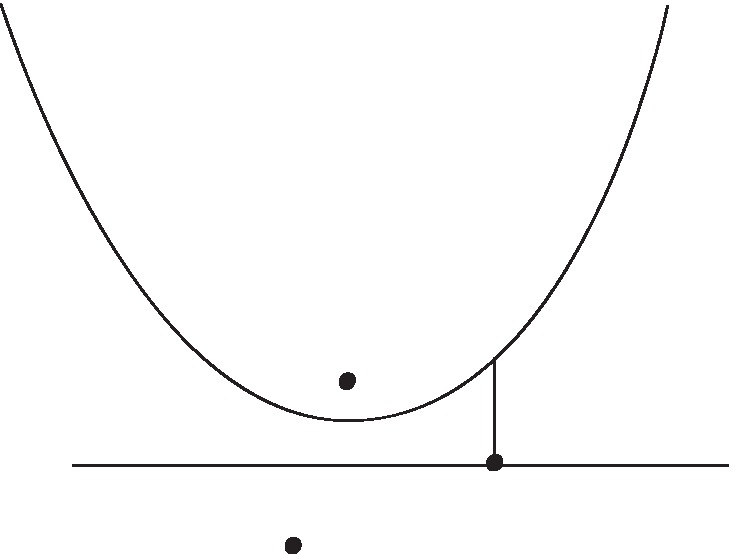
\includegraphics{voronoistep1.jpg}
 \caption{\textbf{Figure 1}. Site events create parabolas on beachfront.}
 \label{fig:step1}
\end{center}
\end{figure}


During the line sweep, two parabolas could pass through each other on the beachfront. There are two cases that could happen. In the first case, one parabola passes ``through'' another. The claim is that this cannot happen. The second case will be described below as a circle event.

\textbf{Claim}:
A parabola cannot pass completely through another parabola.
\begin{proof}
    Consider the time when inner becomes tangent with outer. Inner parabola has higher focus, so descends slower than outer, so the parabola doesn't cross the farther parabola.
\end{proof}

\begin{figure}[h]
\begin{center}
 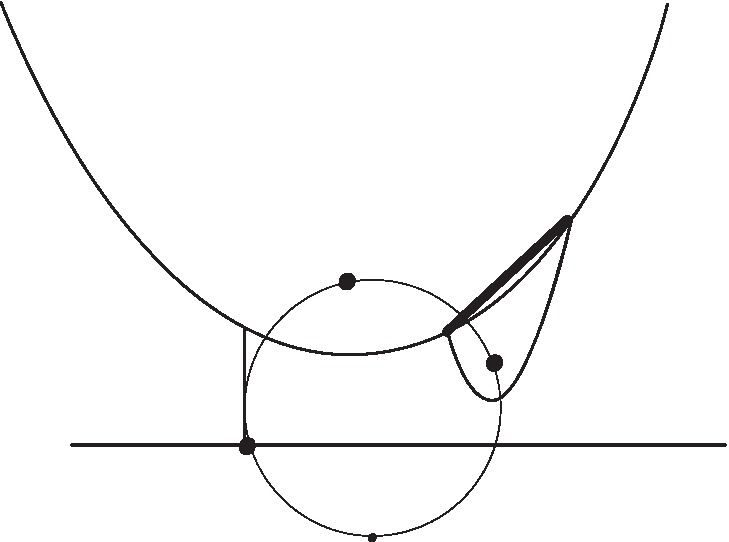
\includegraphics{voronoistep2.jpg}
 \caption{\textbf{Figure 2}. Site events create a future circle event point ahead of sweep line, shown here as a smaller point. Parabolic intersections trace out the voronoi regions, shown here as the thicker line segment.}
\label{fig:step2}
\end{center}
\end{figure}

\subsubsection{Circle event:}

When a new parabola intersects with the intersection of two existing parabolas, a Voronoi vertex is created. See Figure \ref{fig:step3} for details.

 \begin{figure}[h]
 \begin{center}
 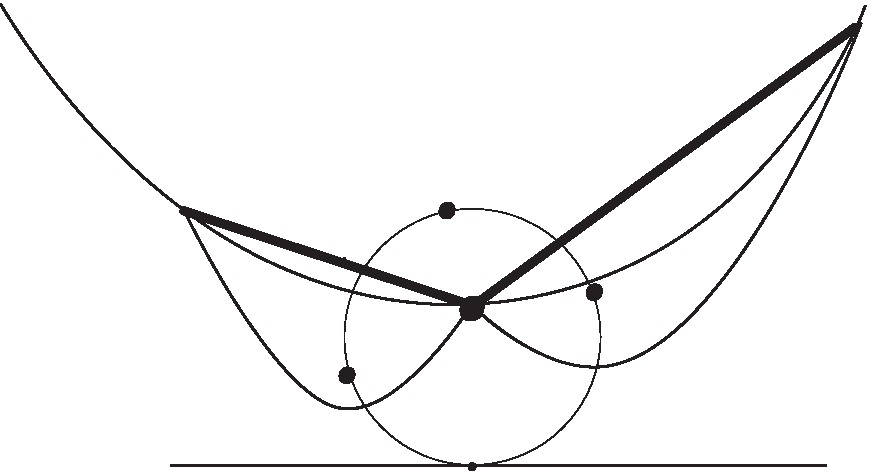
\includegraphics{voronoistep3.jpg}
 \caption{\textbf{Figure 3}. Circle events destroy parabolas on beachfront and create a voronoi vertex, shown here as a larger point.}
 \label{fig:step3}
 \end{center}
 \end{figure}

During a circle event, the parabola hits the intersection of two other parabolas.  All three foci equidistant from intersect "circle event".

The middle parabola cannot ``absorb'' intersection because its focus is higher, so descends slower. 
can emit intersection point at that time, middle parabola disappears from beachfront forever.

\subsubsection{Analysis}
The total number of events is $\leq 2n$, since each parabola corresponding to a point is created and destroyed only once. When we insert or remove a relevant parabola, we must check newly adjacent parabolas for circle events which takes $O(1)$ time. We also compute center of 3 foci's (circle).

Work per event is $O(\log n)$, thus the total runtime is $O(n \log n)$.


\end{document}
